\documentclass{article}
\usepackage{tikz}
\usepackage[a4paper]{geometry}
\usepackage{fancyhdr}
\pagestyle{fancy}
\lhead{Potenz}
\rhead{Januar 2026}
\begin{document}
\section{Potenz}
Die \emph{Potenz} eines Lebewesens gibt an, wie gut ein Lebewesen (bei der Anwesenheit von bestimmten Umweltfaktoren) überleben und sich fortpflanzen kann.
 
Graphisch dargestellt wird diese in einer \emph{Toleranzkurve}.
 
Jedes Lebewesen hat in Bezug auf einen bestimmten Umweltfaktor ein \emph{Optimum}, an welchem es am besten überleben und sich fortpflanzen kann. In der Nähe des Optimums liegt der \emph{Präferenzbereich}. An den Enden des \emph{Toleranzbereiches}, dem Bereich, in welches das Lebewesen überhaupt überleben kann, liegen \emph{Pessima}, gefolgt von jeweils dem \emph{Minimum} oder beziehungsweise dem \emph{Maximum}. 
 
\subsection{Die physiologische und ökologische Potenz}
Es gibt eine physiologische und eine ökologische Potenz.
\begin{description}
 \item[physiologisch] Die Potenz eines Lebewesens unter Laborbedingungen. Andere Umweltfaktoren, welche nicht gemessen werden sollen, werden dabei völlig ausgeblendet.
 \item[ökologisch] Die Potenz unter echte Bedingungen. Andere Umweltfaktoren, z.\,B. Konkurrenz, werden hier nicht ausgeblendet.
\end{description}  
 
\subsection{Euryöken und Stenöken}
Tierarten können in \emph{euryöken} und \emph{stenöken} unterteilt werden. Euryöke Arten haben dabei einen größeren Toleranzbereich. Stenöke Arten spezialisieren sich auf eine bestimmte Art von Umwelt.
 
\subsection{Toleranzkurve}
Eine Toleranzkurve ist ein Diagramm, welches auf der $x$-Achse einen bestimmten Umweltfaktor und auf der $y$-Achse die dazugehörige Potenz eines Lebewesens darstellt.
 
In dieser können alle relevanten Werte sehr einfach ungefähr abgelesen werden.  
\begin{center} 
 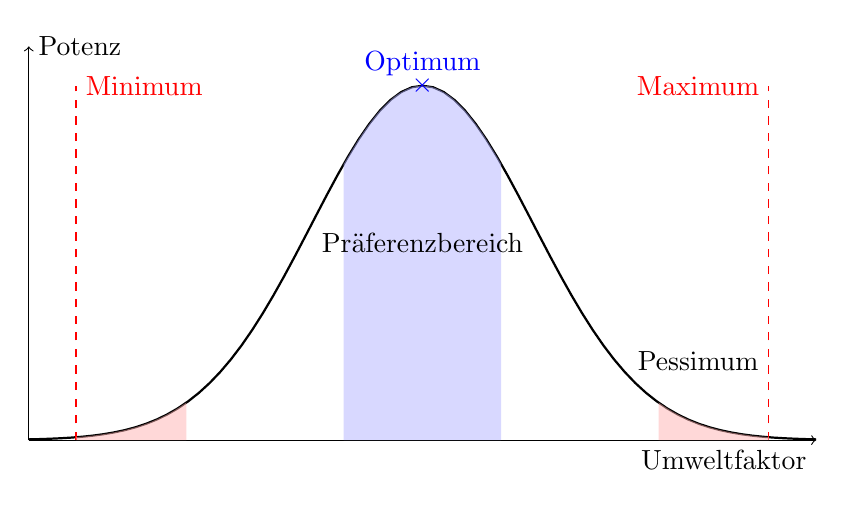
\begin{tikzpicture}     
  \draw[thick, domain=-5:5, samples=75] 
            plot (\x, {4.5*exp(-0.5*\x*\x*0.5)});
     
  \draw[->] (-5,0) -- (5,0) node[below left] {Umweltfaktor};
  \draw[->] (-5,0) -- (-5,5) node[right] {Potenz}; 
    
  \draw[dashed, red] (-4.4,0) -- (-4.4, 4.5) node[right] {Minimum};    
  \draw[dashed, red] (4.4,0) -- (4.4, 4.5) node[left] {Maximum};
 
  \fill[blue!30, opacity=0.5] (-1,0) -- plot[domain=-1:1, smooth, samples=10] (\x, {4.5*exp(-0.5*\x*\x*0.5)}) -- (1,0) -- cycle;
  
  \draw[blue] (0,4.5) node {$\times$} node[above] {Optimum};
  \node[] at (0,2.5) {Präferenzbereich};
 
  \fill[red!30, opacity=0.5] (-4.4,0) -- plot[domain=-4.4:-3, smooth, samples=10] (\x, {4.5*exp(-0.5*\x*\x*0.5)}) -- (-3,0) -- cycle;  
  \fill[red!30, opacity=0.5] (3,0) -- plot[domain=3:4.4, smooth, samples=10] (\x, {4.5*exp(-0.5*\x*\x*0.5)}) -- (4.4,0) -- cycle;
 
  \node[] at (3.5, 1) {Pessimum};
 \end{tikzpicture} 
\end{center}
 
Wird ein zweiter Umweltfaktor hinzugefügt, so liegt ein Ökogramm vor. Hier sind sowohl der $x$-Achse als auch der $y$-Achse Umweltfaktoren aufzufinden. Im Graphen sind selbst dann basierend auf dieser Umweltfaktoren diejenigen Bereiche eingezeichnet, in welchen ein Lebewesen ohne Konkurrenz, gegen Konkurrenz, besonders gut, und so weiter überleben kann kann.
\end{document}